\documentclass{clbeamer2024}

\usepackage{minted}

\usepackage{minted}
\setminted{
	breaklines=true,
	frame=single,
	bgcolor=lightgray,
	fontsize=\small,
	escapeinside=||
}

\usepackage{xcolor}
\definecolor{bg}{rgb}{0.95, 0.95, 0.92} % Couleur gris clair

\title{
	%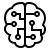
\includegraphics[width=0.5cm]{logos/IA1.png} \hfill
        Introduction à l'Intelligence Artificielle (IA)
	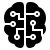
\includegraphics[width=0.5cm]{logos/IA2.png} \hfill
}
\subtitle{Comprendre les bases de l'IA et ses applications}
\author{Slimani Mohamed Amine}
\institute{EHTP}
\date{\today}

\begin{document}
	\setcounter{framenumber}{-1}
	\frame{\titlepage}
	
	
	
	% Sommaire
	\begin{frame}{Sommaire}
		\tableofcontents
	\end{frame}
	
	\section{Qu'est-ce que l'Intelligence Artificielle ?}
	\begin{frame}{Qu'est-ce que l'Intelligence Artificielle ?}
		\begin{itemize}
			\item \textbf{Définition} : L'IA est la capacité d'une machine à imiter l'intelligence humaine, en apprenant, en raisonnant, et en s'adaptant.
			\item \textbf{Domaines de l'IA} :
			\begin{itemize}
				\item \textbf{Apprentissage automatique (Machine Learning)} : Les machines apprennent à partir de données.
				\item \textbf{Traitement du langage naturel (NLP)} : Comprendre et générer du langage humain.
				\item \textbf{Vision par ordinateur} : Analyser et interpréter des images.
			\end{itemize}
		\end{itemize}
	\end{frame}
	
	
	\section{Pourquoi l'IA est-elle importante ?}
	\begin{frame}{Pourquoi l'IA est-elle importante ?}
		\begin{itemize}
			\item \textbf{Automatisation} : Automatiser des tâches répétitives et complexes.
			\item \textbf{Prise de décision} : Aider à prendre des décisions basées sur des données.
			\item \textbf{Innovation} : Créer de nouveaux produits et services.
		\end{itemize}
	\end{frame}
	
	
	\section{Types d'IA}
	\begin{frame}{Types d'IA}
		\begin{itemize}
			\item \textbf{IA faible (ANI)} : Systèmes conçus pour des tâches spécifiques (ex : reconnaissance d'images).
			\item \textbf{IA forte (AGI)} : Systèmes capables de raisonner et d'apprendre comme un humain (encore théorique).
		\end{itemize}
	\end{frame}
	
	
	\section{Techniques d'IA}
	\begin{frame}{Techniques d'IA}
		\begin{itemize}
			\item \textbf{Apprentissage supervisé} : Apprendre à partir de données étiquetées.
			\item \textbf{Apprentissage non supervisé} : Découvrir des patterns dans des données non étiquetées.
			\item \textbf{Apprentissage par renforcement} : Apprendre par essais et erreurs avec des récompenses.
		\end{itemize}
	\end{frame}
	
	
	\section{Applications de l'IA}
	\begin{frame}{Applications de l'IA}
		\begin{itemize}
			\item \textbf{Santé} : Diagnostic médical, découverte de médicaments.
			\item \textbf{Finance} : Détection de fraudes, trading algorithmique.
			\item \textbf{Transports} : Véhicules autonomes, gestion du trafic.
		\end{itemize}
	\end{frame}
	
	
	\section{Exemple de modèle d'apprentissage automatique}
	\begin{frame}{Exemple de modèle d'apprentissage automatique}
		\begin{enumerate}
			\item Collecter et prétraiter les données.
		\item Choisir un modèle (ex : régression linéaire, réseau de neurones).
			\item Entraîner le modèle sur les données.
			\item Évaluer et déployer le modèle.
		\end{enumerate}
	\end{frame}
	
	
	\section{Bonnes pratiques}
	\begin{frame}{Bonnes pratiques}
		\begin{itemize}
			\item \textbf{Qualité des données} : Utiliser des données propres et représentatives.
			\item \textbf{Éviter le surapprentissage (overfitting)} : Utiliser des techniques de régularisation.
			\item \textbf{Éthique} : Respecter la vie privée et éviter les biais.
		\end{itemize}
	\end{frame}
	
	\section{Outils pour travailler avec l'IA}
	\begin{frame}{Outils pour travailler avec l'IA}
		\begin{itemize}
			\item \textbf{TensorFlow} : Bibliothèque open-source pour le machine learning.
			\item \textbf{PyTorch} : Bibliothèque de machine learning développée par Facebook.
			\item \textbf{Scikit-learn} : Bibliothèque Python pour le machine learning.
		\end{itemize}
	\end{frame}
	
	
	
	
	
	
	\section{Pourquoi c'est important ?}
	\begin{frame}{Pourquoi c'est important ?}
		\begin{itemize}
			\item L'IA est une technologie clé pour l'automatisation, la prise de décision, et l'analyse de données.
			\item Elle est utilisée dans de nombreux domaines, tels que la santé, la finance, et les transports.
			\item Comprendre les bases de l'IA est essentiel pour les développeurs et les professionnels de la technologie.
		\end{itemize}
	\end{frame}
	
	\begin{frame}{Résumé}
		\textbf{L'Intelligence Artificielle} est une technologie clé pour l'automatisation, la prise de décision, et l'analyse de données.  
		Explorez, apprenez, et innovez avec l'IA !
	\end{frame}
	
	

	
	
\end{document}
